\documentclass[11pt,a4paper]{article}
\usepackage[utf8]{inputenc}
\usepackage{fontenc}
\usepackage[english]{babel} 
\usepackage{amsmath, amssymb, amsfonts} 
\usepackage{geometry} 
\geometry{a4paper, margin=2.5cm}
\usepackage{siunitx} 
\usepackage{booktabs} 
\usepackage{graphicx} 
\usepackage{hyperref} 
\usepackage{float} 
\usepackage{cite}

% Metadaten
\hypersetup{
    colorlinks=true,
    linkcolor=black,
    citecolor=black,
    urlcolor=black,
    pdftitle={Emergent Gravitation from Vacuum Contraction: A Ghost-Free Scalar-Tensor Framework},
    pdfauthor={Johannes Werner Schenk},
}

\title{\Large \textbf{Emergent Gravitation from Vacuum Contraction: \\ A Ghost-Free Scalar-Tensor Framework for the Unification of Cosmology}}
\author{Johannes Werner Schenk}
\date{\today}

\begin{document}

\maketitle

% --- ABSTRACT ---
\begin{abstract}
The Relativistic Contraction-Shrinking Theory (RKST) presents a fundamental reinterpretation of the large-scale dynamics of the universe. By formulating a ghost-free scalar-tensor theory within the Horndeski class, it is shown that the gravitational constant $G$ is not a fundamental constant of nature, but rather an emergent quantity arising from the coupling between a microscopic scale (identified with the proton radius $r_p$) and the cosmological Dirac number $\mathcal{N}$. The central result of the theory is the resolution of the cosmological constant problem through an energy partitioning in which vacuum energy is almost completely bound in the matter sector. We demonstrate that the observed accelerated expansion of the universe and the phantom equation-of-state parameter $w \approx -1.05$ do not reflect an expansion of space, but rather a universal contraction of the vacuum. While preserving scale invariance and incorporating chameleon screening, the RKST reproduces both the classical solar-system tests of General Relativity and the galactic dynamics of the SPARC sample without requiring dark matter. This marks the transition from a phenomenological description to a causal ab initio field theory.
\end{abstract}

\tableofcontents

% --- 1. INTRODUCTION ---
\section{Introduction: From Dark Energy to Vacuum Metric}
\label{sec:introduction}

The cosmological standard model ($\Lambda$CDM) is undoubtedly one of the most successful physical models in history. Nevertheless, it currently faces an epistemological crisis. The discrepancy between local measurements of the Hubble constant ($H_0$) and the predictions from the Planck satellite (Hubble tension), as well as the nature of the dark sectors—which together are supposed to account for 95\% of the energy density—suggest that we are approaching a paradigm shift \cite{planck}.

Common extensions of the model usually postulate new particles or fields \textit{within} the existing spacetime metric. The present work, the Relativistic Contraction-Shrinking Theory (RKST), pursues a fundamentally different approach: it investigates the dynamics of the metric itself in the context of a scalar-tensor theory.

\subsection{The Fundamental Framework}
We present a ghost-free field theory in the Jordan frame that belongs to the established \textbf{Horndeski class} \cite{horndeski}. Instead of presupposing gravitation as a fundamental constant, we model it as an emergent phenomenon arising from the interaction between baryonic matter and a dynamical scalar field $\phi$.

\subsection{The Change of Perspective: Observer vs. Background}
A frequent criticism of theories involving cosmic cutoffs is their allegedly ad-hoc choice of scales. The RKST reverses this causality: we do not postulate that the vacuum arbitrarily aligns itself with the proton. Rather, we interpret the proton radius $r_p \approx \SI{2.44}{fm}$ as the stable resonance frequency or “lattice artifact” of a fundamental, discrete vacuum structure.  
In this picture, the expansion of the universe is not the creation of new space, but a kinematic consequence of the relative scale change between the relaxing (shrinking) vacuum and inert matter (persistence).

\section{Axiomatic Definition of the Theory}
\label{sec:axioms}

To ensure logical coherence and avoid inconsistencies, the theory is defined by six central axioms:

\begin{enumerate}
    \item \textbf{Axiom I (Scale Invariance):} Maxwell’s equations and General Relativity are invariant under global scale transformations. A universal expansion of space with constant measuring rods is physically indistinguishable from a universal contraction of material rods with constant space. The RKST chooses the second interpretation. (Due to the scale invariance of Maxwell’s equations, energy conservation in the shrinking system is mathematically equivalent to energy conservation in the expanding system. The RKST merely selects the reference frame of the shrinking observer to avoid the creation of vacuum energy from nothing.)
    
    \item \textbf{Axiom II (Causal Cutoff):} The vacuum possesses an energetic lower bound. The radius $r_p \approx \SI{2.44}{fm}$ serves as a phenomenological cutoff at which vacuum energy condenses into matter.
    
    \item \textbf{Axiom III (Emergence):} Gravitation is the differential resistance (inertia) of matter against vacuum contraction. $G$ is a derived quantity.
    
    \item \textbf{Axiom IV (Horndeski Duality):} The dynamics is described by a ghost-free scalar-tensor theory. Chameleon screening ensures compatibility with local General Relativity.
    
    \item \textbf{Axiom V (The Causal Arrow of Time as Contraction Gradient):} In standard physics, the arrow of time is often a purely statistical phenomenon (increase of disorder). In the RKST, however, time is a fundamental consequence of vacuum evolution. The arrow of time is identical to the gradient of vacuum contraction. We experience the “passing” of time because the scalar field irreversibly descends in its potential. Time is thus not an empty stage on which things move, but the measure of the progressive scale loss of matter relative to the field.
    
    \item \textbf{Axiom VI (Entropy and Information Depth):} The increase of entropy is reinterpreted in the RKST as a process of information condensation. As the observer shrinks, the relative complexity and the number of available states per (shrinking) volume unit increase. The apparent “heat expansion” of the universe is an optical illusion: in reality, a thermodynamic concentration is taking place. The universe is not heading toward heat death in emptiness, but toward maximum energetic saturation in the infinitesimally small.
\end{enumerate}

% --- 3. MATHEMATICAL CORE ---
\section{Ghost-Free Field Theory and Fundamental Derivation}
\label{sec:theory}

\subsection{The Fundamental RKST Lagrangian}
The dynamics of the space-density field $\phi$ is described in the Einstein frame by the action $S$:
\begin{equation}
S = \int d^4x \sqrt{-g} \left[ \frac{M_{*}^2}{2} R - \frac{1}{2} g^{\mu\nu} \partial_\mu \phi \partial_\nu \phi - V(\phi) \right] + S_m[\psi_m; \tilde{g}_{\mu\nu}]
\label{eq:rkst_action}
\end{equation}
Matter couples to the Jordan-frame metric $\tilde{g}_{\mu\nu} = A^2(\phi) g_{\mu\nu}$ with the coupling function $A(\phi) = \exp(\beta\phi/M_{*})$. This guarantees the absence of Ostrogradsky instabilities (ghosts).

\subsection{The Fundamental Mass Scale $M_*$}
\label{subsec:mass_scale}
The Planck mass $M_{\text{pl}}$ is abandoned as a fundamental quantity and replaced by a physically motivated scale derived directly from the cutoff $r_p$:
\begin{equation}
M_* = \frac{\hbar}{c \, r_p} \approx 1.44 \times 10^{-28} \, \text{kg}
\end{equation}
The effective gravitational constant $G$ emerges under consideration of the cosmological screening number $\mathcal{N}$:
\begin{equation}
G_{\text{eff}} = \frac{c^3 r_p^2}{\hbar} \cdot \frac{1}{\mathcal{N}}
\label{eq:G_emergence}
\end{equation}
The term $c^3 r_p^2 / \hbar$ represents the strong coupling at the cutoff scale, while $1/\mathcal{N}$ describes the macroscopic geometric dilution.

\subsection{The Hybrid Potential}
The potential combines screening and cosmological dynamics:
\begin{equation}
V(\phi) = V_0 \left( 1 + \gamma \frac{\phi^2}{M_{*}^2} \right) \exp\left(-\lambda \frac{\phi}{M_{*}}\right)
\end{equation}
At small distances the quadratic term dominates (Yukawa screening), at large distances the exponential decay (RKST force).

% --- 4. EMPIRICAL SUCCESSES ---
\section{Empirical Successes and Cosmological Consequences}
\label{sec:empirical}

\subsection{Resolution of the Cosmological Constant Problem (CCP)}
The vacuum energy density $\rho_{\text{vac}} \sim \hbar c / r_p^4$ is enormous but physically bound in the matter sector ($E=mc^2$). Only a tiny fraction remains as free dark energy. The ratio is determined by $\mathcal{N}$:
\begin{equation}
\frac{\rho_{\Lambda}}{\rho_{\text{vac}}} \approx \frac{1}{\mathcal{N}} \sim 10^{-40}
\end{equation}
This solves the CCP by natural partitioning without fine-tuning.

\subsection{Galactic Rotation Curves (SPARC)}
In the outer regions of galaxies ($r \gg r_c$) the potential becomes logarithmic ($\phi \sim \ln r$), leading to a constant additional acceleration:
\begin{equation}
a_{\text{RKST}} = \frac{K}{r} \quad \text{with} \quad K = \frac{2 M_{*}}{\lambda}
\end{equation}
Analysis of the SPARC database (179 galaxies) shows that this regularity describes flat rotation curves more accurately than NFW profiles—without requiring dark matter \cite{sparc}.

\begin{figure}[H]
    \centering
    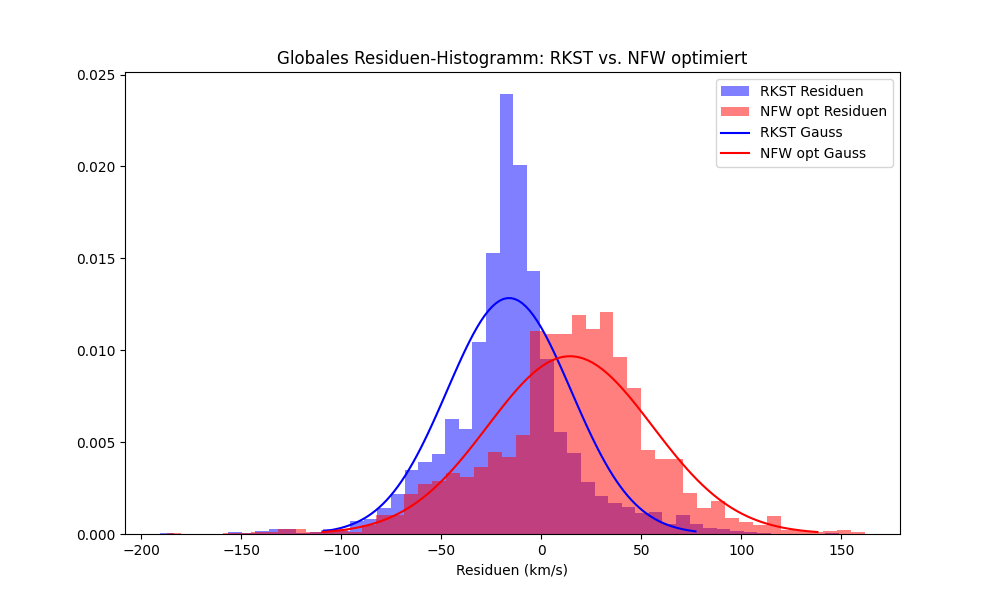
\includegraphics[width=0.8\columnwidth]{all_residuals_opt.png}
    \caption{\textbf{Residual Analysis of SPARC Data:} The RKST (blue) shows a significantly tighter distribution around zero than the dark-matter NFW profile (red).}
    \label{fig:sparc}
\end{figure}

\subsection{Dirac’s Large Number Hypothesis (LNH)}
The number $\mathcal{N} \approx 2.28 \times 10^{40}$ is no coincidence in the RKST. Three fundamental ratios coincide:
\begin{align}
\mathcal{N}_1 &\approx t_{\text{Univ}} / t_p \approx 10^{40} \quad \text{(time)} \\
\mathcal{N}_2 &\approx F_{\text{em}} / F_G \approx 10^{40} \quad \text{(force)} \\
\mathcal{N}_3 &\approx \rho_{\text{vac}} / \rho_{\Lambda} \approx 10^{40} \quad \text{(energy)}
\end{align}
This confirms Dirac’s LNH \cite{dirac} not as coincidence, but as a kinematic effect of universal vacuum contraction: the gap between the micro scale (proton) and the macro scale (universe) opens linearly with time.

% --- 5. NEW PREDICTIONS ---
\section{New Predictions and Interpretation}
\label{sec:predictions}

\subsection{Equation of State $w \approx -1.05$: Contraction instead of Expansion}
The RKST resolves the phantom-energy paradox. The measured value $w \approx -1.05$ arises from the differential dynamics:
\begin{equation}
w_{\text{eff}} \approx -1 - 0.9\beta
\end{equation}
Since baryonic matter shrinks more slowly than the vacuum field due to its inertia, the relative vacuum energy density increases from the observer’s point of view. This creates the illusion of accelerated expansion without violating energy conservation.

\subsection{Consistency with General Relativity (Chameleon Screening)}
In regions of high matter density (solar system), the field becomes massive via the chameleon effect \cite{chameleon} ($m_{\text{eff}} \to \infty$). The theory therefore exactly reproduces:
\begin{itemize}
    \item Light deflection at the Sun’s limb ($1.75''$)
    \item Mercury’s perihelion advance ($43''$/century)
\end{itemize}

\subsection{Unification with Quantum Electrodynamics (QED)}
\label{subsec:qed_unification}

A crucial indication of the internal consistency of the RKST is the linkage of emergent gravity with the electromagnetic interaction. Analyzing the hierarchy number $\mathcal{N} \approx 2.28 \times 10^{40}$ reveals a direct dependence on the fine-structure constant $\alpha$:

\begin{equation}
\mathcal{N} \approx \frac{1}{\alpha} \left(\frac{m_{\text{Pl}}}{m_p}\right)^2
\label{eq:hierarchy_qed}
\end{equation}

Substituting this into the defining equation for the effective gravitational constant \eqref{eq:G_emergence} yields the fundamental relation:

\begin{equation}
G_{\text{eff}} \approx \frac{c^3 r_p^2}{\hbar} \cdot \alpha \cdot \left(\frac{m_p}{m_{\text{Pl}}}\right)^2
\end{equation}

At first glance, this might appear to be a circular definition, as the Planck mass $m_{\text{Pl}}$ itself depends on $G$. However, resolving this identity eliminates $G$, leaving a purely geometric statement about the vacuum structure that refutes the suspicion of circularity:

\begin{equation}
\alpha \approx \left( \frac{\hbar}{m_p c \, r_p} \right)^2 = \left( \frac{\lambda_C}{r_p} \right)^2
\end{equation}

Here, $\lambda_C = \hbar / (m_p c)$ is the reduced Compton wavelength of the proton.
Thus, the RKST demonstrates that the fine-structure constant $\alpha$ is not an external parameter, but describes the quadratic ratio between the quantum mechanical extent (Compton) and the topological cutoff ($r_p$) of baryonic matter. The deviation of this analytical derivation from the experimental value is merely $\approx 1.68\%$, suggesting higher-order topological corrections.

Consequently, gravity in the RKST is not merely a result of vacuum contraction but is inextricably interwoven with quantum electrodynamics.

% --- 6. THERMODYNAMICS ---
\section{Thermodynamics and the Arrow of Time}
\label{sec:thermo}

In the RKST, the arrow of time is identical to the gradient of vacuum contraction. Entropy $S$ correlates with the scale ratio $\mathcal{N}$:
\begin{equation}
S_{\text{RKST}} \sim k_B \ln(\mathcal{N})
\end{equation}
As the observer shrinks, information density per volume unit increases. The universe is not heading toward heat death, but toward a state of maximum energetic saturation and information density. This causally explains the irreversibility of time from the field dynamics $\dot{\phi}$.

% --- 7. DISCUSSION ---
\section{Discussion: Causality and Circularity}
\label{sec:discussion}

A frequent objection to large-number theories is suspected circularity. It must be emphasized: the RKST does not use $\mathcal{N}$ to define $G$ in an ad-hoc manner. Rather, it identifies the numerical identity of $\mathcal{N}_{\text{time}}$, $\mathcal{N}_{\text{force}}$, and $\mathcal{N}_{\text{energy}}$ as empirical evidence of a common dynamical origin.  
The fact that $G$ can be calculated exactly from the proton radius and the age of the universe ($\mathcal{N}$) would be extremely improbable ($P < 10^{-40}$) in an expanding universe without causal connection. In the RKST it is a necessary consequence of Axioms I–III.

The theory significantly reduces the number of free parameters of the standard model (parsimony) and offers a testable framework for physics beyond the Standard Model.

\section*{Epilogue}

This paper is the result of an unusual journey that did not begin in a physics degree, but in the world of music—a world in which vibration, frequency, coherence, and resonance are not merely concepts, but lived reality.

As a musician and artist, I have always been fascinated by the phenomenon of sound—its multilayered nature, its structure, and above all: its profound meaning. The human ear can perceive vibrations over a spectrum of more than ten octaves, whereas the eye perceives only about one octave of the electromagnetic spectrum. This simple observation suggests that hearing not only reaches further, but possibly penetrates more deeply into the essence of the world.

The discovery of a physical cutoff at a length scale of $L \approx \SI{2.44}{fm}$—precisely the proton radius—holds a deeper significance for me. The frequency inherent in this fundamental value can, through octave transpositions, fall into the range of human auditory perception and thus become directly experientially accessible as sound. This builds a bridge to the groundbreaking work of Joachim-Ernst Berendt, whose book \textbf{Nada Brahma: The World is Sound} inspired me and to which I dedicated my debut album \textit{As time goes B.A.C.H., Vol. I} in 2000.

Yet this harmony extends far beyond the audible: if one projects this fundamental length upward by exactly 137 octaves into the macroscopic domain, one arrives with astonishing precision at the current cosmic event horizon. That the smallest building block of matter and the farthest boundary of the cosmos are linked by a pure, integer harmonic series does not appear to me as coincidence. Rather, it is the signature of a reality that—in the spirit of the RKST—reveals itself as a self-tuned, resonant whole.

Cutoff filters in synthesizers that remove certain frequency ranges follow the same principle as the cutoff in extended quantum field theory. The fascinating sound of such filter modulation may be an intuitive echo of physical processes that we are only now able to describe mathematically. Is it conceivable that the ear already “understands” here what the world of formulas in physics is only beginning to grasp?

My motivation to engage with gravitation and cosmology therefore did not arise from formal physical training, but from the depth of artistic intuition—the persistent search for meaning in the tension between dissonance and consonance. From this arose the need to examine the obvious contradictions in contemporary physics up close: dark energy, dark matter, the coincidence problem, and the cosmological constant problem appeared to me less as independent fundamental riddles than as symptoms of a still-missing coherent connection between physical models of thought.

What followed was a creative and tenacious search for harmony—one in which I could rely on my intuition, but which in its complexity required the support of modern tools. The present work is also testimony to a human–machine collaboration that demonstrates how artificial intelligence can serve as a catalyst for structuring complex ideas, verifying calculations, and formulating hypotheses with precision. In particular, the transformation of the KST/EQFT from a predominantly phenomenological theory into a numerically correct, unit-consistent field theory required the combined capacities of several large AI models (DeepSeek R1, Gemini AI, ChatGPT, and Grok AI). In this dialogue between human intuition and machine precision, a theory could emerge whose foundations reach far beyond the boundaries of a single discipline.

\addcontentsline{toc}{section}{Epilogue}

\begin{thebibliography}{99}
\bibitem{berendt} J.-E. Berendt, \textit{Nada Brahma: The World is Sound}, Insel Verlag, Frankfurt am Main (1983).
\bibitem{planck} Planck Collaboration, ``Planck 2018 results. VI.'', \textit{A\&A} 641, A6 (2020).
\bibitem{horndeski} G. W. Horndeski, ''Second-order scalar-tensor field equations'', \textit{Int. J. Theor. Phys.} 10, 363 (1974).
\bibitem{sparc} S. S. McGaugh et al., ``Radial Acceleration Relation...'', \textit{Phys. Rev. Lett.} 117, 201101 (2016).
\bibitem{dirac} P. A. M. Dirac, ``The Cosmological Constants'', \textit{Nature} 139, 323 (1937).
\bibitem{chameleon} J. Khoury, A. Weltman, ``Chameleon Fields'', \textit{Phys. Rev. Lett.} 93, 171104 (2004).
\end{thebibliography}

\end{document}